\documentclass[journal]{IEEEtran}
\usepackage{german}
\usepackage[T1]{fontenc}
\usepackage[utf8]{inputenc}
%\usepackage{cite}
\usepackage{graphicx}
\graphicspath{{./pdf/}{./figs/}}
\DeclareGraphicsExtensions{.pdf,.jpg,.png}
\usepackage[cmex10]{amsmath}
\usepackage{amsfonts}
\usepackage{algorithmic}
\usepackage{array}
%\usepackage{mdwmath}
%\usepackage{mdwtab}
\usepackage{eqparbox}
\usepackage[tight,footnotesize]{subfigure}



%\usepackage[caption=false]{caption}
%\usepackage[font=footnotesize]{subfig}
\usepackage{fixltx2e}
\usepackage{stfloats}
\usepackage{url}
\hyphenation{op-tical net-works semi-conduc-tor}

\begin{document}
\title{Sampling Based Motion Planning}
\author{André~Groß,~\IEEEmembership{Student~B.Sc.~Informatik,~JG-Universität~Mainz}}%
% The paper headers
\markboth{Handout zum Computergraphik Seminar am 11. Jannuar 2013}%
{test... \MakeLowercase{\textit{et al.}}}

\maketitle


\begin{abstract}
Die Sampling basierte Bewegungsplanung beschäftigt sich mit der Planung von Bewegungen in Höherdimensionalen Räumen. Sie kommt genau dann zum Einsatz, wenn die Konstruktion des Konfigurationsraumes mit einem Vollständigen Bewegungsplaner nicht möglich (PSPACE) oder zeitkritisch ist.

In diesem Seminarvortrag wollen wir uns mit der Sampling Based Motion Planning im allgemeinen beschäftigen. In diesem Zuge werden wir uns den Probablistic Road Map Algorithmus genauer an sehen und herausfinden wie man eine Kugel zufällig im Raum orientieren kann.
Abschließend soll noch ein Ausblick auf eine aktuelle Open Source Bibliothek gegeben werden.
\end{abstract}

\IEEEpeerreviewmaketitle



\section{Einführung}
\IEEEPARstart{M}{otion Planning} (MP) oder zu deutsch Bewegungsplanung wird benötigt, wenn man innerhalb eines Raumes einen Weg zwischen einem Start- und Zielzustand finden möchte.
Hauptanwendungsgebiet der MP ist im Bereich Robotik.

Die MP kann man grundsätzlich in zwei Bereiche unterteilen. Der Erste wäre die Combinatorial Motion Planning (Kombinatorische Bewegungsplanung). Die Algorithmen des zweiten Bereiches werden unter Sampling-Based Motion Planning (Stichproben Basierte Bewegungsplanung) zusammengefasst.

Hierzu eine kleine Übersicht ausgewählter Algorithmen:
\begin{itemize}
\item Combinatorial Motion Planning
\begin{itemize}
\item Cell Decomposition
\item Computational Algebraic Geometry
\end{itemize}
\item Sampling-Based Motion Planning
\begin{itemize}
\item Tree Based
\item Probablistic Road Map
\end{itemize}
\end{itemize}
\cite{lavalle06}
\cite{arvo00}
\cite{tsk07}
\subsection{Das Problem}
Der gegebene Raum besteht aus blockierten Bereichen und freien.
\[\mathcal C = \mathcal C_{free} + \mathcal C_{blocked}\]

Wir wollen nun einen Pfad $p$ zwischen Start- und Zielzustand durch den freien Raum finden.
\[q_{start},q_{goal}\in \mathcal C_{free}\]
\[p:[0,1]\rightarrow \mathcal C_{free}\]

mit
\[p(0)=q_{start},p(1)=q_{goal}\]\cite{tsk07}
\subsection{Combinatorial Motion Planning}
Die kombinatorische Bewegungsplanung besteht aus exakten und somit vollständigen Algorithmen. Diese Kerneigenschaften führen dazu, dass ich die Möglichkeit habe mit diesen die sichere Aussage treffen zu können ob überhaupt ein Weg existiert. 
\cite{lavalle06}
\cite{tsk07}
\subsubsection{Cell Decomposition}
Hier baut man den Konfigurationsraum auf, indem man den freien Raum in Zellen unterteilt. Der einfachste Ansatz ist hier die Vertical Cell Decomposition, bei der man in einer Richtung den freien Raum in Parallelogramme unterteilt und damit einen Graphen aufbaut. Die anschließende Wegfindung ist dann nur noch eine Suche auf dem Graphen. Die Abbildungen \ref{cell1} und \ref{cell2} erläutern dies weiter.
\cite{lavalle06}
\begin{figure}[!t]
\centering
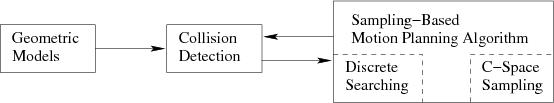
\includegraphics[width=2.5in]{img2115}
\caption{Vertical Cell Decomposition Graph}
\label{cell1}
\end{figure}
\begin{figure}[!t]
\centering
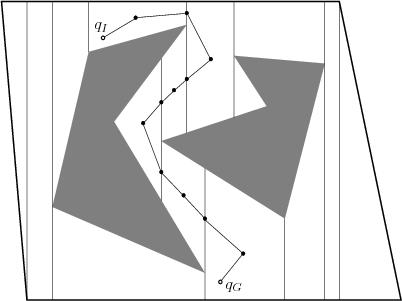
\includegraphics[width=2.5in]{img2116}
\caption{Beispielpfad}
\label{cell2}
\end{figure}
\subsubsection{Computational Algebraic Geometry}
Hier versucht man mit algebraischen Mitteln, typischerweise in höherdimensionalen Räumen, das Problem der Wegfindung zu lösen.
\cite{lavalle06} Ohne weiter darauf ein zu gehen möchte ich hier als Beispiel die Ermitlung des Schnittpunktes zweier paralleler Geraden anmerken. 
\subsection{Sampling-Based Motion Planning}
Komplexitätsanalysen haben gezeigt, dass die Wegfindung mit Mitteln der Kombinatorik PSPACE-Vollständig ist.\cite{Rei79}\cite{Can88} Dies bedeutet dass der Speicherbedarf polinomiell wächst. Da die Wegfindung jedoch oft zeitkritischer Natur ist, versuchte man sich an schnelleren, wahrscheinlichweitsorientierten Verfahren. \cite{BL91}\cite{KSLO96} 

Die Idee ist hierbei auf eine explizite Konstruktion des Konfigurationsraumes zu verzichten. Man versucht nun durch zufälliges ausprobieren mögliche Konfigurationen zu finden. Hierzu benötigt man eine gute Kollissionserkennung, deren Funktionsweise nun nicht mehr für die Planung von Belang ist.

\begin{figure}[!t]
\centering
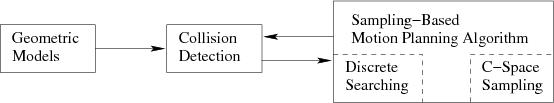
\includegraphics[width=2.5in]{img1670}
\caption{Kapselung der Bewegunguplanung}
\label{mp1}
\end{figure}

Damit kann man nun den Algorithmus unabhängig der zu Grunde liegenden Geometrie betrachten. Siehe Abb. \ref{mp1}
\cite{lavalle06}

Diese Algorithmen haben jedoch nur eine wahrscheinlichkeitstheoretische Vollständigkeit und besitzen somit nur die Möglichkeit eine Lösung zu finden. Existiert hingegen keine Lösung, so terminieren sie auch nicht. \cite{KLMR98}
\subsubsection{Tree based}
\begin{figure}[!t]
\centering
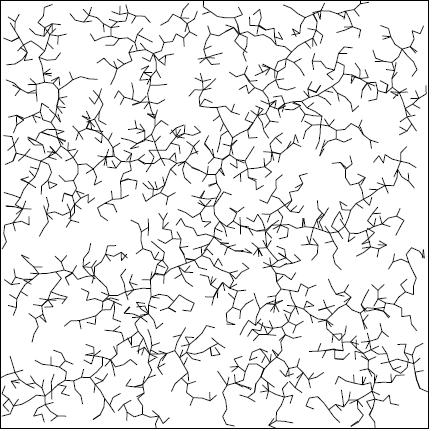
\includegraphics[width=2.5in]{RRT}
\caption{RRT Beispiel}
\label{rrt}
\end{figure}
Die Baum basierten Algorithmen bauen ausgehend von einem Saatpunkt aus einen Baum auf, welcher den Konfigurationsraum räpresentiert. In Abbildung \ref{rrt} ist ein Beispiel für einen RRT angegeben.
\cite{tsk07}
\section{Probablistic Road Map}
\begin{figure}[!t]
\centering
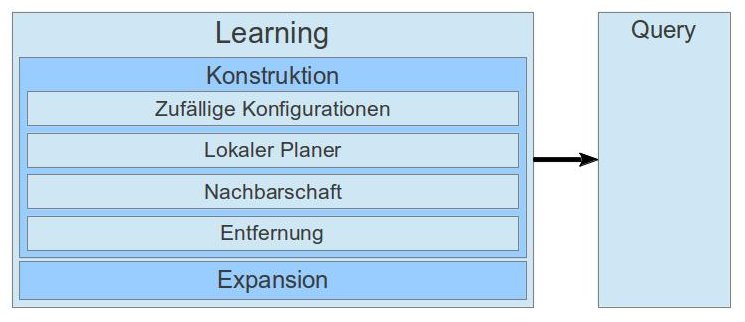
\includegraphics[width=2.5in]{prm}
\caption{RRT Beispiel}
\label{prmphases}
\end{figure}
\subsection{Lern- Phase}
\subsubsection{Konstruktion}
\paragraph{Zufällige Konfiguration}
\paragraph{Lokaler Planer}
\paragraph{Nachbarschaft}
\paragraph{Entfernung}
\subsubsection{Expansion}
\subsection{Abfrage Phase}

\section{Uniform Random Rotation}
\section{Open Motion Planning Library}


\hfill André Groß
 
\hfill \today

\subsection{Subsection Heading Here}
Subsection text here.

\section{Abschluss}
The conclusion goes here.

\appendices
\section{equation}
ee

\section{}
nn

\section*{Danksagung}
Dem Auditorium möchte ich für seine Aufmerksamkeit danken.

Rainer für das immer offene Ohr und die guten Quellen. Sebastian Limbach für sein Buch und die Starthilfe bei den Random Rotations.

Herrn Prof. Dr. Schömer für seine Unterstützung und die Möglichkeit des Seminares.


\begin{thebibliography}{1}

\bibitem{lavalle06}Steven M. LaValle, \emph{Planning Algorithms}.Copyright 2006
   Cambridge University Press, 842 pages, ISBN-13: 978-0521862059.

\bibitem{arvo00} James Arvo, \emph{Fast Random Rotation Matrices}. Program of Computer Gaphics, Gem, Cornell University.

\bibitem{tsk07}
Konstantinos I. Tsianos, Ioan A. Sucan, Lydia E. Kavraki, \emph{Sampling-Based Robot Motion Planning:
Towards Realistic Applications}. In Computer Science Review, August, Volume 1, Issue 1, p. 2–11, 2007.

\bibitem{BL91} J. Barraquand and J.-C. Latombe. \emph{Robot motion planning :
A distributed representation approach}. International Journal of
Robotics Research, 10(6):628–649, 1991.

\bibitem{Rei79} H. J. Reif.  \emph{Complexity of the mover’s problem and generalizations}.
In IEEE Symposium on Foundations of Computer Science, 1979.

\bibitem{KLMR98} L. E. Kavraki, J.-C. Latombe, R. Motwani, and P. Raghavan.
 \emph{Randomized query processing in robot path planning}. Journal of
Computer and System Sciences, 57(1):50–60, 1998.

\bibitem{Can88} J. Canny.  \emph{Some algebraic and geometric computations in pspace}. In
Annual ACM Symposium on Theory of Computing, pages 460–469,
Chicago, Illinois, United States, 1988. ACM Press.

\bibitem{KSLO96} L. E. Kavraki, P. Svestka, J.-C. Latombe, and M. Overmars.
 \emph{Probabilistic roadmaps for path planning in high dimensional
configuration spaces}. IEEE Transactions on Robotics and
Automation, 12(4):566–580, August 1996.

\bibitem{tbm} http://virtual-labs.ac.in/labs/cse17/RRT/RRT.html

\bibitem{HH02} S. Hirsch and D. Halperin.  \emph{Hybrid motion planning: Coordinating
two discs moving among polygonal obstacles in the plane}. In WAFR,
pages 225–241, Nice, 2002.

\bibitem{HY98} D. Halperin and C.-K. Yap.  \emph{Combinatorial complexity of translating
a box in polyhedral 3-space}. Computational Geometry: Theory and
Applications, 9:181–196, 1998.

\bibitem{LaV98} S. M. LaValle.  \emph{Rapidly-exploring random trees: A new tool for path
planning}. Technical Report 11, Computer Science Dept., Iowa State
University, 1998.

\bibitem{LK01} S. M. LaValle and J. J. Kuffner.  \emph{Randomized kinodynamic planning}.
International Journal of Robotics Research, 20(5):378–400, May 2001.

\end{thebibliography}

\end{document}


